\documentclass[12pt, a4paper, twoside]{article}
\usepackage[utf8]{inputenc}
\usepackage[cm]{fullpage}
\usepackage{fancyhdr}
\usepackage{textcomp}
\usepackage{graphicx}
\usepackage{commath}
\usepackage[portuguese]{babel}
\usepackage{float}
\usepackage{hyperref}
\usepackage{amsmath}
\usepackage{amssymb}

\title{Relatório do experimento 5 de LDCE}

\begin{document}

\maketitle

\section{Questão 1}

\begin{figure}[H]
    \centering
    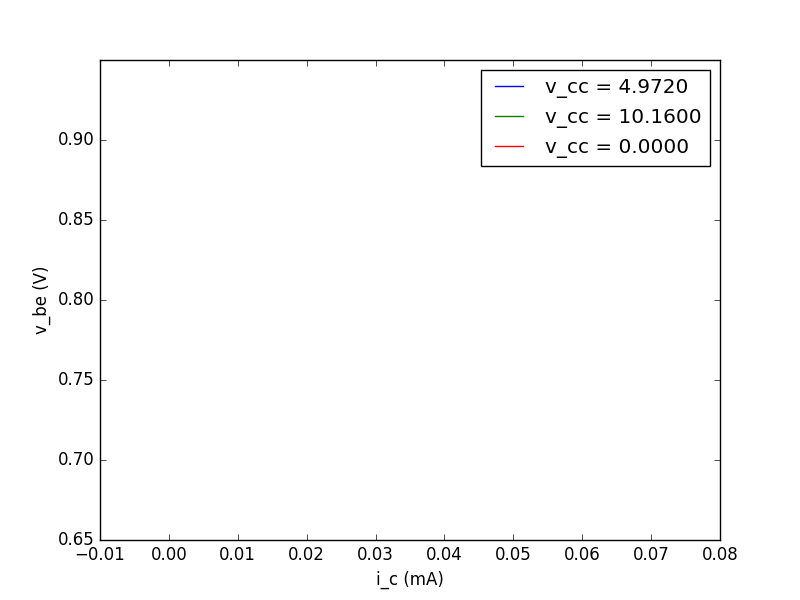
\includegraphics[width=0.6\textwidth]{figs/rel5/v_be.png}
    \caption{Gráfico da corrente $I_C$ em função de $V_{BE}$.}
\end{figure}

Por esta curva, é fácil ver quando o transistor está operando em regime de corte e quando ele está operando em seu modo ativo: quando a tensão $V_{BE}$ está abaixo do limiar $V_T = 0,5V$, a corrente $I_C = 0A$ sempre, ou seja, o transistor está em corte. Caso contrário, observamos uma curva que aparentemente está decaindo, indicando que, para tensões maiores, poderíamos até ver o comportamento do transistor em saturação. De toda forma, para $V_{BE} > V_{T}$, já há passagem de corrente, indicando que o transistor opera em regime ativo.

\begin{figure}[H]
    \centering
    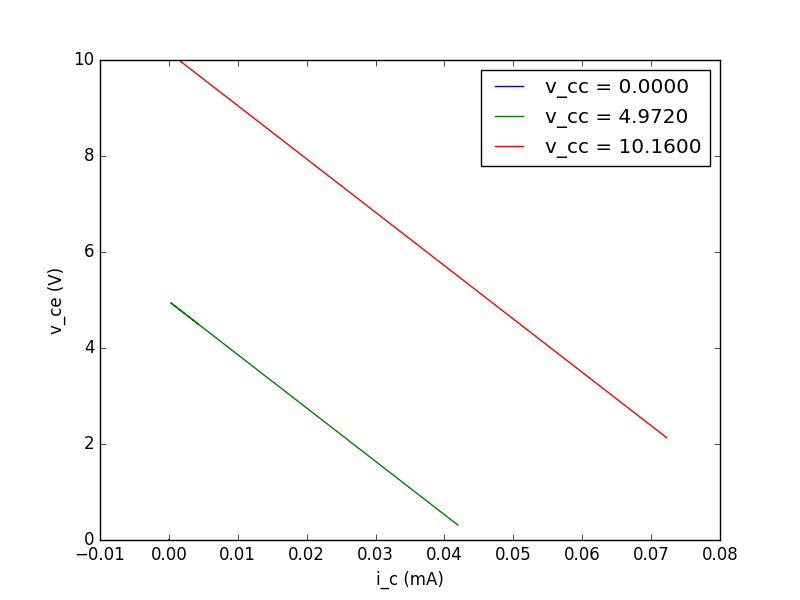
\includegraphics[width=0.6\textwidth]{figs/rel5/v_ce.png}
    \caption{Gráfico da corrente $I_C$ em função de $V_{CE}$.}
\end{figure}

O primeiro comentário acerca da curva $I_C\ x\ V_{CE}$ é que não há passagem de corrente, isto é $I_C = 0A$, quando a tensão $V_{CE} = 0V$, o que é esperado, já que não há tensão no emissor para poder gerar um corrente e, consequentemente, alimentar o dispositivo. Todavia, quando há alimentação para o coletor, notamos que a corrente diminui com o aumento da tensão. Isso acontece pois a corrente $I_C$ depende da queda de tensão no resistor $R_E$, e, pela de Ohm, esses valores tem que se compensar já que a resistência deste componente é constante.

\end{document}
